% Document Set-Up
\documentclass[12pt, letterpaper]{aiaa-tc}

\usepackage{graphicx}
\graphicspath{{Graphics/}}

\usepackage{amsmath}

\usepackage{bm}

\usepackage{xcolor}
\definecolor{navy}{RGB}{0, 0, 139}

\usepackage{titlesec}

\title{Project 2: Maneuver Reconstruction}
\author{Tyson Warner and Jack Pence}
\date{November 12, 2023}

\setlength{\parskip}{1em}

\begin{document}

\renewcommand\thesection{\Roman{section}}
\titleformat{\section}[hang]
  {\fontsize{12pt}{12.4pt}\color{navy}\bfseries}
  {\thesection.}
  {0.5em}
  {}

\maketitle

% \newpage

\section{PROJECT STATEMENT: MANEUVER RECONSTRUCTION}

Maneuver reconstruction is an important part of the astrodynamics suite of applications. Specially in sparse data
environments, or in the event that teh spacecraft is performing multiple maneuvers, identifying how much delta-v
was expended is an important metric in characterizing the capabilities of a satelltie. In this project, we will idealize
a simplified maneuver reconstruction experiment.

Consider a spacecraft that is continuously being tracked. The ground station looses tracking when a maneuver
is performed, but has regained its custody at a later time. (Maneuver detection and tracking is another important
and difficult problem in astrodynamic. For this project, let us assume that this problem is solved). A schematic of
one such maneuver reconstruction is shown as follows:

\begin{figure}[h]
    \centering
    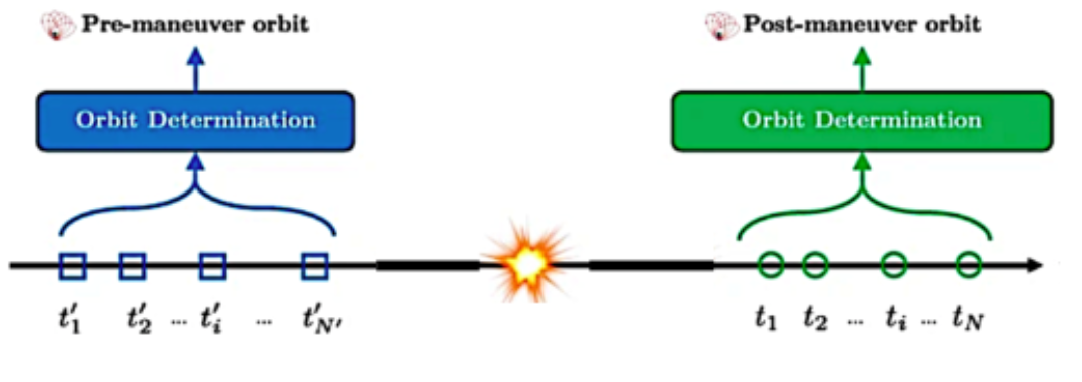
\includegraphics[width=0.75\textwidth]{maneuver_reconstruction_schematic}
    \caption{Maneuver Reconstruction Schematic.}
    \label{fig:maneuver_reconstruction_schematic}
\end{figure}

We will utilize Gauss' initial orbit determination to identify the orbit that the spacecraft occupies before and
after the maneuver and calculate how much delta-v was used to transfer between them.


\section{ANALYTICAL PART: COMPUTING THE MANEUVER}

Given the pre-maneuver and post-maneuver orbit parameters, compute the delta-v used to transfer from one to the
other. Let us assume a coplanar case for this project, i.e. the inclination and RAAN of the pre and post-maneuver
orbit are the same. However, the argument of perigee may be different.

In such a case, let us suppose that we adopt the perifocal reference frame for the first ellipse. In this reference
frame, then, the argument of periapsis of the second ellipse is rotated counter-clockwise from the x-axis by an
angle $\Delta\omega$ - where $\Delta\omega$ is the difference in the argument of periapsis of the two co-planar orbits.

So, the radial distance of a satellite on the first orbit can be thought of as:
\begin{equation}
    r_1=\frac{p_1}{1+e_1 cos(f)}
    \label{eq:orbitequation1}
\end{equation}
and that on the second orbit is:
\begin{equation}
    r_2=\frac{p_2}{1+e_2 cos(f-\Delta\omega)}
    \label{eq:orbitequation2}
\end{equation}
If the two orbits intersect, the two radial distances must be equal:
\[ r_1=r_2=r \]
Our aim in this analytical part of the project is to find the value of the radius where the two orbits intersect. This
leads to a quadratic equation in the free variable $r$. Let's go about this step-by-step.

\raggedright \textit{A. Derivation of radius of intersecting orbits}
\begin{enumerate}
    
    \item Using the first relation:
    \[ r_1=\frac{p_1}{1+e_1 cos(f)} \]
    rearrange to identify an expression for $cos(f)$. Also, using trigonometric identities, identify an expression for
    $r^{2}sin^{2}(f)$. We will keep these quantities aside, as we will be using them at a later step.
    
    \textbf{SOLUTION:}
    
    Using $r_1=r$ and solving for $cos(f)$:
    \begin{equation}
        cos(f)=\frac{1}{e_1}\left (\frac{p_1}{r}-1 \right)
        \label{eq:cosf}
    \end{equation}
    Solving for $r^2sin^2(f)$ using Pythagoras' theorem ($sin^2(f)=1-cos^2(f)$) and squaring the previous, rearranged expression:
    \[ r^2sin^2(f) = r^2(1-cos^2(f)) \]
    \[ r^2sin^2(f) = r^2\left (1- \left(\frac{1}{e_1}\left (\frac{p_1}{r}-1 \right)\right)^2 \right) \]
    Expanding this expression (this will be helpful for step 5):
    \begin{equation}
        r^2sin^2(f) = \left(\frac{e_1^2-1}{e_1^2}\right)r^2+\left(\frac{2p_1}{e_1^2}\right)r+\left(-\frac{p_1^2}{e_1^2}\right)
        \label{eq:r^2sin^2f_1}
    \end{equation}
    \item Using the relation:
    \[ r_2=\frac{p_2}{1+e_2 cos(f-\Delta\omega)} \]
    rearrange to identify an expression for $cos(f-\Delta\omega)$

    \textbf{SOLUTION:}

    Repeat the first part of step 1 but replacing subscripts and substituting $cos(f-\Delta\omega)$ for $cos(f)$:
    \begin{equation}
        cos(f-\Delta\omega)=\frac{1}{e_2}\left (\frac{p_2}{r}-1 \right)
        \label{eq:cos(f-dw)}
    \end{equation}
    \item Expand the above expression using the trigonometric identity for $cos(A-B)$
    and rearrange to find an expression for $rsin(f)$. After this step, you may also substitute the expression for 
    $cos(f)$ from step 1.
    \\On performing this step, you should find the resulting expressions contain the terms:
    \[ \alpha=e_2cos(\Delta\omega)-e_1 \]
    \[ \beta=e_1p_2-e_2p_1cos(\Delta\omega) \]
    \[ \gamma=e_1e_2sin(\Delta\omega) \]
    you may use these placeholder variables ($\alpha$, $\beta$, $\gamma$) to simplify your math process.

    \textbf{SOLUTION:}

    Expanding the resulting expression from Equation~\eqref{eq:cos(f-dw)} and solving for $sin(f)$:
    \[ cos(f-\Delta\omega)=cos(f)cos(\Delta\omega)-sin(f)sin(\Delta\omega) \]
    \[ sin(f)=\frac{cos(f-\Delta\omega)-cos(f)cos(\Delta\omega)}{sin(\Delta\omega)} \]
    Multiplying $r$ to both sides:
    \[ rsin(f)=r\left(\frac{cos(f-\Delta\omega)-cos(f)cos(\Delta\omega)}{sin(\Delta\omega)}\right) \]
    Substituting the results from steps 1 and 2:
    \[ rsin(f)=r\left(\frac{\frac{1}{e_2}\left (\frac{p_2}{r}-1 \right)-\frac{1}{e_1}\left (\frac{p_1}{r}-1 \right)cos(\Delta\omega)}{sin(\Delta\omega)}\right) \]
    Simplifying by factoring out $\frac{1}{r}$ in the numberator and multiplying the numberator and denominator by $e_1$ and $e_2$:
    \[ rsin(f)=\left(\frac{e_1(p_2-r)-e_2(p_1-r)cos(\Delta\omega)}{e_1e_2sin(\Delta\omega)}\right) \]
    \[ rsin(f)=\left(\frac{(e_2cos(\Delta\omega)-e_1)r+e_1p_2-e_2p_1cos(\Delta\omega)}{e_1e_2sin(\Delta\omega)}\right) \]
    Substituting for the placeholder variables mentioned earlier in this step:
    \begin{equation}
        rsin(f)=\frac{\alpha r+\beta}{\gamma}
        \label{eq:rsinf}
    \end{equation}
    \item Now, you may square the resulting expression on either side to obtain another expression for 
    $r^2sin^2(f)$ i.e., you will obtain an expression as:
    \[r^2sin^2(f)= \]
    
    \textbf{SOLUTION:}
    
    Squaring both sides of the resulting expression from Equation~\eqref{eq:rsinf}:
    \[ r^2sin^2(f)=\frac{(\alpha r+\beta)^2}{\gamma^2} \]
    Expanding this expression (this will be helpful for the next step):
    \begin{equation}
        r^2sin^2(f)=\frac{\alpha^2}{\gamma^2}r^2+2\frac{\alpha\beta}{\gamma^2}r+\frac{\beta^2}{\gamma^2}
        \label{eq:r^2sin^2f_2}
    \end{equation}
    \item  Plug in your relation for $r^2sin^2(f)$ from step 1. At this stage, we have eliminated true anomaly from the equations.

    \textbf{SOLUTION:}

    Equating the results for $r^2sin^2(f)$ from Equation~\eqref{eq:r^2sin^2f_1} and Equation~\eqref{eq:r^2sin^2f_2}:
    
    \[ \left(r^2sin^2(f)\right)_{step 1}=\left(r^2sin^2(f)\right)_{step 4} \]
    \begin{equation}
        \left(\frac{e_1^2-1}{e_1^2}\right)r^2+\left(\frac{2p_1}{e_1^2}\right)r+\left(-\frac{p_1^2}{e_1^2}\right)=\left(\frac{\alpha^2}{\gamma^2}\right)r^2+\left(\frac{2\alpha\beta}{\gamma^2}\right)r+\left(\frac{\beta^2}{\gamma^2}\right)
        \label{eq:full_solve_for_r}
    \end{equation}
    \item You will notice that you have a quadratic expression in $r$.
    \[ ar^2+br+c=0 \]
    Collect the terms that multiply $r^2$, $r$, and the constant term, i.e. $a$, $b$, $c$. These are the coefficients you will
    use to compute the roots of a quadratic equation:
    \[ r=\frac{-b\pm\sqrt{b^2-4ac}}{2a} \]
    As the final step, you should obtain something of the form:
    \[ a=\frac{e_1^2-1}{e_1^2}-\frac{\alpha^2}{\gamma^2} \]
    \[ b=\frac{2p_1}{e_1^2}-\frac{2\alpha\beta}{\gamma^2} \]
    \[ c=-\left(\frac{p_1^2}{e_1^2}+\frac{\beta^2}{\gamma^2}\right) \]

    \textbf{SOLUTION:}

    Collecting terms from Equation~\eqref{eq:full_solve_for_r}:
    \[ \left(\frac{e_1^2-1}{e_1^2}\right)r^2+\left(\frac{2p_1}{e_1^2}\right)r+\left(-\frac{p_1^2}{e_1^2}\right)=\left(\frac{\alpha^2}{\gamma^2}\right)r^2+\left(\frac{2\alpha\beta}{\gamma^2}\right)r+\left(\frac{\beta^2}{\gamma^2}\right) \]
    \[ \left(\frac{e_1^2-1}{e_1^2}-\frac{\alpha^2}{\gamma^2}\right)r^2+\left(\frac{2p_1}{e_1^2}-\frac{2\alpha\beta}{\gamma^2}\right)r+\left(-\left(\frac{p_1^2}{e_1^2}+\frac{\beta^2}{\gamma^2}\right)\right)=0 \]
    Equating the previous result to a quadratic expression with constants $a$, $b$, and $c$ $\left(a^2r+br+c=0\right)$:
    \[ a=\frac{e_1^2-1}{e_1^2}-\frac{\alpha^2}{\gamma^2} \]
    \[ b=\frac{2p_1}{e_1^2}-\frac{2\alpha\beta}{\gamma^2} \]
    \[ c=-\left(\frac{p_1^2}{e_1^2}+\frac{\beta^2}{\gamma^2}\right) \]
\end{enumerate}

\raggedright \textit{B. Testing the algorithm}

Now, consider two sets of orbital elements of two spacecraft:


\begin{table}[h]
    \centering
    \begin{tabular}{|l|l|l|}
    \hline
                        & Orbit 1 & Orbit 2  \\ \hline
    semimajor axis (km) & 13000   & 7226.58  \\
    eccentricity        & 0.3     & 0.444819 \\
    inclination (deg)   & 20      & 20       \\
    RAAN (deg)          & 30      & 30       \\
    AOP (deg)           & 50      & 301.901  \\ \hline
    \end{tabular}
\end{table}

\begin{enumerate}
    \item Identify the radius at the intersecting point.
    
    \textbf{SOLUTION:}

    Calculating semi-latus rectum (in km) using given eccentricities and semimajor axes for orbits 1 and 2 ($p_1$ and $p_2$ respectively):
    \[ p_n=a_n\left(1-e_n^2\right) \]
    \[ p_1=13000\left(1-(0.3)^2\right)=11830 \]
    \[ p_2=7226.58\left(1-(0.444819)^2\right)=5796.7 \]
    Calculating the difference in the argument of periapsis ($\Delta\omega$) between the two orbits:
    \[ \Delta\omega=\omega_2-\omega_1=301.901^{\circ} -50^{\circ}=251.901^{\circ} \]
    Calculating the constants from part A, step 3 ($\alpha$, $\beta$, $\gamma$):
    \[ \alpha=e_2cos(\Delta\omega)-e_1=-0.4382 \]
    \[ \beta=e_1p_2-e_2p_1cos(\Delta\omega)=3373.767 \]
    \[ \gamma=e_1e_2sin(\Delta\omega)=-0.1268 \]
    Calculating the constants from part A, step 6 ($a$, $b$, and $c$):
    \[ a=\frac{e_1^2-1}{e_1^2}-\frac{\alpha^2}{\gamma^2}=-22.045 \]
    \[ b=\frac{2p_1}{e_1^2}-\frac{2\alpha\beta}{\gamma^2}=446657.9 \]
    \[ c=-\left(\frac{p_1^2}{e_1^2}+\frac{\beta^2}{\gamma^2}\right)=-2262440535.1 \]
    Calculating the radius using the relation obtained from part A, step 6:
    \[ r=\frac{-b\pm\sqrt{b^2-4ac}}{2a} \]
    where the two possible solutions are $r=10129.35$ km and $r=10131.71$ km. 
    Both values are valid solutions of where the orbits intersect, so we chose to continue
    using $r=10129.35$ km.

    \item Compute the position and velocity vectors at these points on the two orbits. Note, that position vectors will
    be the same, but the velocity vectors may be different.
    
    \textbf{SOLUTION:}
    
    Calculating $cos(f)$ using Equation~\eqref{eq:cosf}:
    \[ cos(f)=\frac{1}{e_1}\left (\frac{p_1}{r}-1 \right)=0.5596 \]
    Calculating $sin(f)$ using Equation~\eqref{eq:rsinf}:
    \[ sin(f)=\frac{\alpha r+\beta}{r\gamma}=0.8287 \]
    Solving for $f$ using a quadrant check between the two relations above:
    \[ f=cos^{-1}(0.5596)=55.9689^{\circ}/-55.9689^{\circ} \]
    \[ f=sin^{-1}(0.8287)=55.9689^{\circ}/124.0311^{\circ} \]
    Using the value that is similar, $f=55.9689^{\circ}$.
    Finding the position vector in the orbital reference frame of the first orbit:
    \[ \vec{r}_{orbital}=[r\quad 0\quad 0]^T=[10129.35\quad 0\quad 0]^T \]
    Calculating the magnitude of angular momentum ($h$) of each orbit ($\mu_e=398600.4418\frac{km^3}{s^2}$):
    \[ h_n=\sqrt{\mu_{e} p_n} \]
    \[ h_1=\sqrt{\mu_{e} p_1}=68669.08 \]
    \[ h_2=\sqrt{\mu_{e} p_2}=48068.36 \]
    There will be two velocity vectors at the intersection, one for each orbit. Calculating 
    the radial and tangential components of each velocity ($v_{r}$ and $v_{\theta}$ respectively) in the orbital 
    reference frame of the first orbit (all in $\frac{km}{s}$):
    \[ v_{r,1}=\frac{h_1}{r}\;\frac{e_1sin(f)}{1+e_1cos(f)}=1.44315 \]
    \[ v_{r,2}=\frac{h_2}{r}\;\frac{e_2sin(f-\Delta\omega)}{1+e_2cos(f-\Delta\omega)}=1.01251 \]
    \[ v_{\theta,1}=\frac{h_1}{r}=6.77922 \]
    \[ v_{\theta,2}=\frac{h_2}{r}=4.74545 \]
    Constructing the velocity vectors in the orbital frame:
    \[ \vec{v}_{orbital,n}=[v_{r,n}\quad v_{\theta,n}\quad 0]^T \]
    \[ \vec{v}_{orbital,1}=[v_{r,1}\quad v_{\theta,1}\quad 0]^T=[1.44315\quad 6.77922\quad 0]^T \]
    \[ \vec{v}_{orbital,2}=[v_{r,2}\quad v_{\theta,2}\quad 0]^T=[1.01251\quad 4.74545\quad 0]^T \]
    Converting the three vectors from orbital frame to inertial (ECI) frame by using 
    a 3-1-3 rotation by angles $(\omega+f)$, $I$, $\Omega$:
    \[ \vec{r}_{orbital}=\bm{C}_{ON}\vec{r}_{ECI} \]
    \begin{equation}
        \vec{r}_{ECI}=\bm{C}^{-1}_{ON}\vec{r}_{orbital}
        \label{eq:DCMtransform}
    \end{equation}
    where $\bm{C}_{ON}$ is:
    \[ \bm{C}_{ON}=
    \begin{bmatrix}
        \cos(\omega+f) & \sin(\omega+f) & 0 \\
        -\sin(\omega+f) & \cos(\omega+f) & 0 \\
        0 & 0 & 1 \\
    \end{bmatrix}
    \begin{bmatrix}
        1 & 0 & 0 \\
        0 & \cos(I) & \sin(I) \\
        0 & -\sin(I) & \cos(I) \\
    \end{bmatrix}
    \begin{bmatrix}
        \cos(\Omega) & \sin(\Omega) & 0 \\
        -\sin(\Omega) & \cos(\Omega) & 0 \\
        0 & 0 & 1 \\
    \end{bmatrix} \]
    $I$ is the inclination, where $I=20^{\circ}$ for both orbits.
    $\Omega$ is right ascension of the ascending node, where $\Omega=30^{\circ}$ for both orbits.
    $f$ is the true anomaly relative to the first orbit, where $f=55.9689^{\circ}$ for both orbits.
    $\omega$ is the argument of perigee, where $\omega_1=50^{\circ}$ for the first orbit and 
    $\omega_2=301.901^{\circ}$ for the second orbit.

    Calculating $\bm{C}^{-1}_{ON}$ for both orbits:
    \[ \bm{C}^{-1}_{ON,1}=
    \begin{bmatrix}
        -0.6900 & -0.7033 & 0.1710\\ 0.6448 & -0.7046 & -0.2962\\ 0.3288 & -0.0941 & 0.9397
    \end{bmatrix}\]
    \[ \bm{C}^{-1}_{ON,2}=
    \begin{bmatrix}
        0.8829 & -0.4373 & 0.1710\\ 0.4694 & 0.8318 & -0.2962\\ -0.0127 & 0.3418 & 0.9397
    \end{bmatrix}\]
    Obtaining position and velocity vectors using equation \eqref{eq:DCMtransform}:
    \[ \vec{r}_{ECI}=\bm{C}^{-1}_{ON}\vec{r}_{orbital}=[-6988.98\quad 6531.78\quad 3330.75]^T \]
    \[ \vec{v}_{ECI,1}=\bm{C}^{-1}_{ON,1}\vec{v}_{orbital,1}=[ -5.76386\quad -3.84599\quad -0.16335]^T \]
    \[ \vec{v}_{ECI,2}=\bm{C}^{-1}_{ON,2}\vec{v}_{orbital,2}=[-4.03629\quad -2.69071\quad -0.11359]^T \]
    \item Compute the delta-v at the intersection point to transfer from one orbit to another.
    
    \textbf{SOLUTION:}
    Calculating the delta-v ($\Delta V$):
    \[ \Delta V=|\vec{v}_{ECI,2}-\vec{v}_{ECI,1}| \]
    \[ \Delta V=|[-1.72757\quad -1.15529\quad -0.04976]^T| \]
    \[ \Delta V=\sqrt{(-1.72757)^2+(-1.15529)^2+(-1.15529)^2} \]
    \[ \Delta V=2.0789\;\frac{km}{s} \]

\end{enumerate}

\section{NUMERICAL PART}
Now that you have performed the analytic part, the numerical part will have you implement an Initial Orbit
Determination Algorithm. The following data has been provided to you:

% include table
In this data,
\begin{enumerate}
    \item The date and time of the observation is recorded
    \item The Azimuth and Elevation values of the satellite expressed in a Topocentric Equatorial Frame are provided
    in degrees
    \item The telescope's position (on the Earth's surface) is provided in the inertial frame in km. You may be interested
    to know that the telescope side is located at latitude = 31.9466 N and longitude = 108.8977 W, which is
    also the proposed location of the Penn State University Dynamical Observatory (PSUDO) lab (check it out
    on Google maps!)
\end{enumerate}
You may also load this data in using the .mat file attached using the matlab command:

\quad load('IODMeasurements.mat')

\raggedright \textit{A. Your tasks are the following:}

\begin{enumerate}
    \item Taking 3 measurements at a time in sequence, perform the Gauss' method of Initial Orbit Determination to
    obtain the value of $\bm{r}_1$, $\bm{r}_2$, and $\bm{r}_3$ of the satellite.
    \item \textbf{Hint: Recall that Gauss' method requires you to find the roots of a 8th degree polynomial. You may
    use the roots() command in matlab to do so.} Also note that Of the 8 roots, 4 are imaginary, and you can
    reject them. But there will be 4 real roots. Negative roots can also be rejected. However, if you obtain three
    positive real roots, you have to now figure out which of the roots is a viable value for $|\bm{r}_2|$. You may need to
    identify all the orbits involved to make this decision.
    \item Using the three position vectors you have obtained by employing the Gauss' method, perform Gibb's method
    to find the position and velocity of the middle measurement. \textit{(Note that there are 24 measurements, so you
    will have to Perform Gauss method 8 times. It may be useful to write a function that does this.)}
    \item Convert this position and velocity pair to orbital elements.
    \item After performing these three tasks above, how many unique orbits do you observe? Enter your answer in the
    following form:
    % include table
    \item Plot all of these orbits in one plot. Just by observation can you identify the potential locations of the delta-v
    maneuvers? Show them on the plot. Also, mark with arrows the direction of motion of your spacecraft.
    \item Finally perform the task you were assigned in the analytic part to identify each delta-v that explains the
    measurements and the orbits you have got. Fill in your answers as follows:
    % include tabe
\end{enumerate}

\end{document}